\chapter{Introducci\'{o}n}

En 1914 Vesto Slipher descubrió que las galaxias espirales rotan. Detectó líneas de absorción inclinadas en el espectro  de las galaxias  M31 y Sobrero \cite{Slipher1914}. Después, Jan Oort en 1932 encontró por primera vez que debe haber tres veces tanta masa como es observado la luz visible, mientras estudiaba movimientos estelares sobre el plano de la Via Láctea. Este descubrimiento le sugirió incluir componentes de medio interestelar no detectado para explicar la masa faltante en este sistema. Observaciones similares para las partes externas de NGC3115 mostró que la razón masa a luz es aproximadamente dos órdenes  de magnitud mayor que en la vecindad solar \cite{Oort40} como evidencia  de materia no visible. Ésto es conocido como el problema de la `masa faltante'; esto es, la masa contenida en objetos brillantes de una región definida en el espacio no corresponde a su masa dinámica que podemos conocer por las interacciones gravitacionales.\\

La razón masa a luz $\Upsilon = M/L$ es una cantidad que describe cuánta masa es una fracción de la luz expresado en unidades solares ($\Upsilon_\odot = \textrm{M}_\odot\textrm{L}_\odot^{-1}$). Esta cantidad ha sido la principal herramienta para investigar el problema de la `masa faltante' en sistemas estelares como la  Vía Lactea, galaxias externas y cúmulos de galaxias.\\

Han surgido algunas explicaciones del problema de la `masa faltante'. H. Babcock en 1939 encontró que la curva de rotación es aproximadamente plana en la periferia  de la galaxia M31 en lugar de la caída Kepleriana dada la disminución de la luminosidad (predicha por el perfil de luminosidad) \cite{Babcock1939}. Él concluyó que la razón masa-luz no debe ser constante en el radio galáctico, pero debe incrementar. Él sugirió dos explicaciones para este fenómeno: la absorción de luz debe incrementar en las partes externas de la galaxia, o se requiere una modificación a la dinámica Newtoniana \cite{Sanders}. \\

Los descubrimientos publicados por Fritz Zwicky \cite{Z33, Z37} sugirieron la existencia de `materia no visible' o materia oscura en sus resultados usando el teorema del virial a las velocidades de galaxias en el cúmulo Coma. Zwicky midió las velocidades radiales de galaxias en el cúmulo, y estimó su masa y por lo tanto la masa promedio de la galaxia. Entonces comparando su valor con la luminosidad, él obtuvo la razón masa a luz de galaxias en el cúmulo $\Upsilon = M/L = 500 \Upsilon_\odot$ sugiriendo que la mayor contribución es materia oscura en el cúmulo. Después, en 1970 Vera Rubin primero reveló una evidencia observacional de materia oscura en la galaxia M31. Ella se dió cuenta que la velocidad circular se vuelve constante en regiones externas de la galaxia basado en su curva de rotación de 67 espectros  H\textsc{ii}  entre un rango en el radio galáctico de (3-24 kpc) \cite{R70}.\\

La curva de rotación de galaxias tipo disco en el principal observable cinemático que permite estudiar propiedades dinámicas de sus estrellas y gas interestelar, en adición a la estructura, procesos de formación e la galaxia \cite{S01}. La forma de las curvas de rotación se relaciona con la morfología de galaxias espirales \cite{R80} buscando una curva de rotación universal dependiendo solo de la luminosidad de la galaxia \cite{P96}, y no solo de la luminosidad sino de una familia multi-parámetro tal como tipo morfológico, la forma de la distribución de luz y otras propiedades ópticas\cite{N07}.\\

La distribución de masa en una componente de una galaxia puede ser estimada por la suposición que la razón masa a luz es constante. Dado que la luminosidad de la galaxia es un observable astrofísico, puede ser obtenido un perfil de luminosidad de una componente y por lo tanto inferir su distribución de masa. Entonces es posible encontrar una curva de rotación para cada contribución de masa y derivar cantidades interesantes como la relación de masas bulbo a disco o disco a materia oscura, o igualmente interesante la extensión radial de cada componente de masa. El modelamiento de la curva de rotación usando descomposición de masa is ampliamente usado en estudios recientes. Esto evidencia la influencia de todas las contribuciones de masa en cada posición, del núcleo hasta décadas en el radio galáctico.\\


\begin{figure}
  \centering
    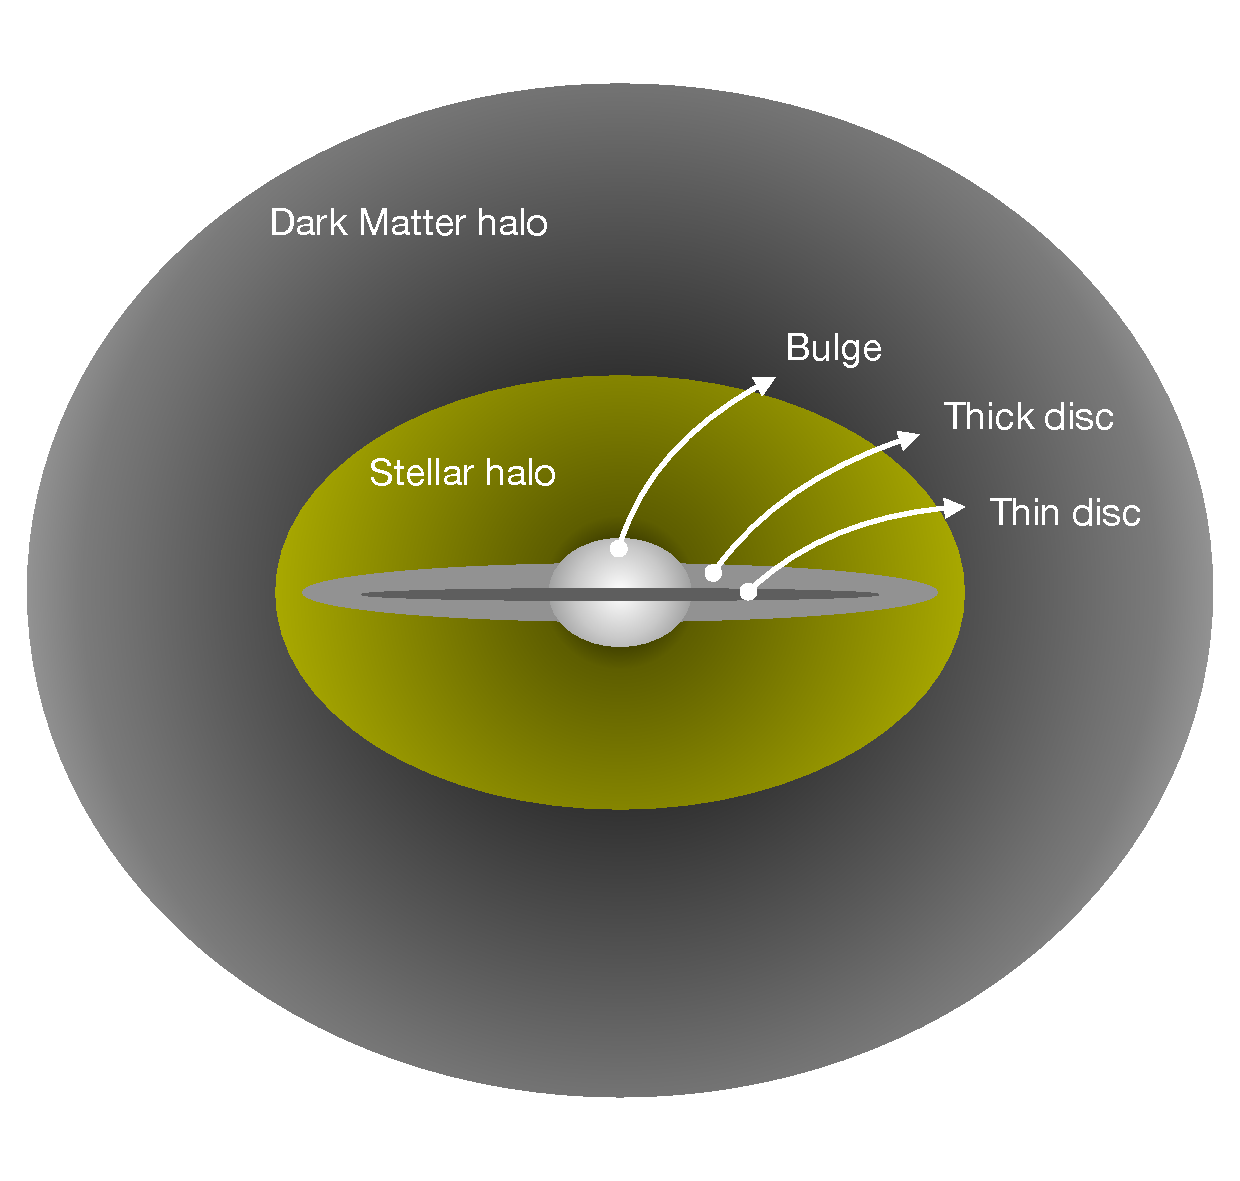
\includegraphics[width=0.95\columnwidth]{Kap1/diagram_disk_galaxy.pdf}
  \caption{ Diagram of the main components of disc-like galaxies: spheroidal bulge, thin and thick discs, spheroidal stellar and Dark Matter halos.}
  \label{fig:Fig_diagram_galaxy}
\end{figure}

El modelo dinámico de una galaxia obtenido de la curva de rotación es un estimativo a primera aproximación, dado que la velocidad circular es muy sensible a perturbaciones impuestas por ejemplo por brazos espirales, disco contra-rotante, movimientos disipativos del gas conocidos como \emph{inflows/outflows}, por lo que se requiere una descripción completa del modelo dinámico. La formulación de las ecuaciones de Jeans y del parámetro de anisotropía de las velocidades dan cuenta del elipsoide de velocidades que permite caracterizar con mayor exactitud el modelo y verificarlo respecto observables astrofísicos como la dispersión de velocidades y el campo de velocidades. La curva de rotación es especialmente precisa en modelar la dinámica a grandes distancias del centro galáctico, pero en la región central la forma de la curva de rotación carece de una definición clara.\\







